\chapter{Regression}
\label{sec:regression}

\section{Architecture Details}

\subsection*{Studies with Large Sample Windows}

The studies in this section were performed using the full large window samples, of size 51x51x25 in ECAL and 11x11x60 in HCAL.
%\footnote{/eos/project/d/dshep/LCD/DDHEP/*Escan\_*\_MERGED/}.
The samples consist of approximately 800,000 events for each particle type.  2/3 of the events were used for training and 1/3 of the events were used for testing.

The most important design choice found for the DNN/CNN networks is the size of the window used as input.  For both DNN and CNN, to achieve the best performance for energies above 150~GeV, a minimum $(x,y)$ size of 25x25 in the ECAL and 5x5 in the HCAL is needed.  For energies below 150~GeV, the optimal performance is observed for a window size of 51x51 in the ECAL and 11x11 in the HCAL.  This is presumably due to wider showers at low energy.  The impact of the choice of window size is shown for DNN in Figure~\ref{fig:reg_dnn_numcells}, with the results for CNN being similar.  Drawbacks to the larger window size, however, include larger files, more memory usage, and that training takes about 5 times longer per epoch.

\begin{figure}[htbp]
\centering
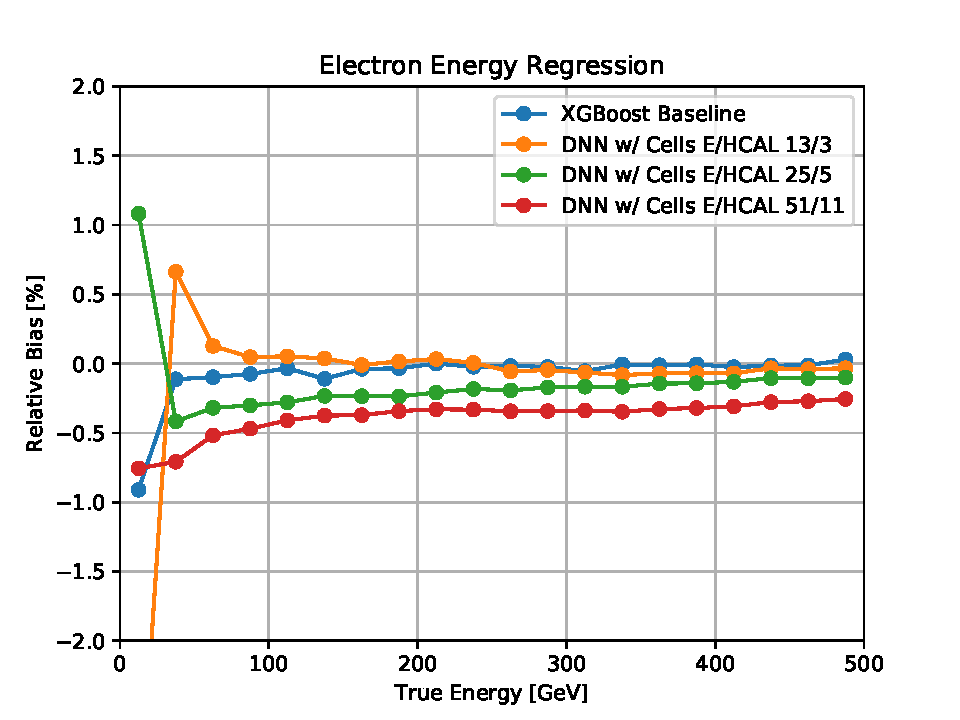
\includegraphics[width=0.38\textwidth]{Images/Calo/bias_vs_E_EleFixed_nn_numcells_zoom.pdf}
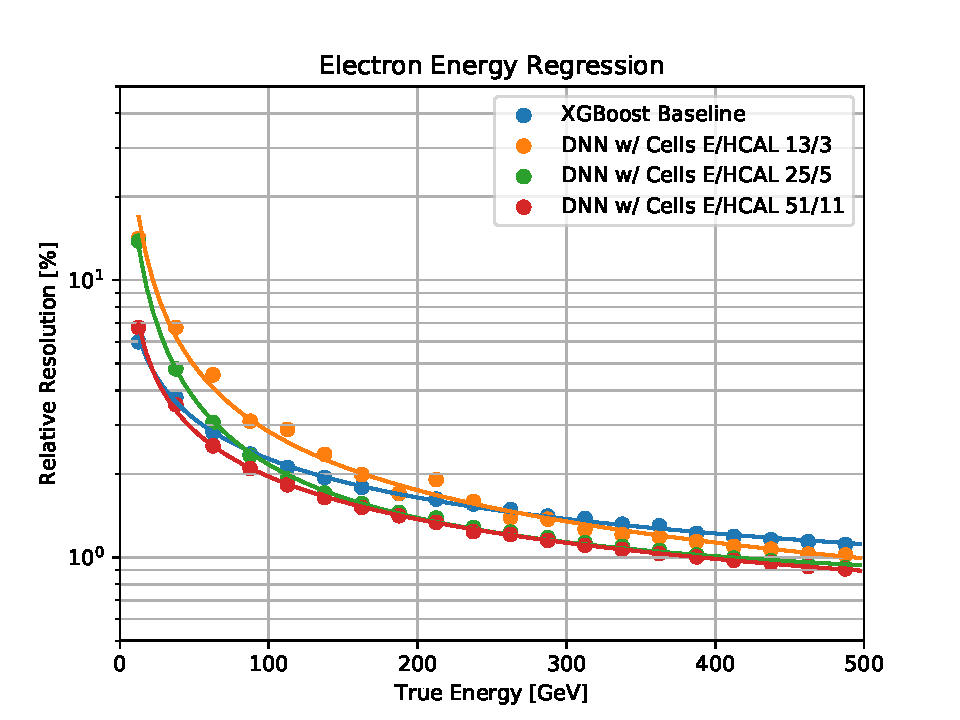
\includegraphics[width=0.38\textwidth]{Images/Calo/res_vs_E_EleFixed_nn_numcells_fits.pdf}
\caption{Bias (top) and resolution (bottom) as a function of true energy for DNN energy predictions for electrons, with varying input window sizes.
}
\label{fig:reg_dnn_numcells}
\end{figure}

Showers for \chpi\ were observed to be wider than the other particle types, especially at low energies, and so we compare the effect of the calorimeter window size choice for \chpi\ in Figure~\ref{fig:reg_nn_numcells_chpi_large_window}.  The wider window of 51x51 in $(x,y)$ in the ECAL and 11x11 in the HCAL gives better performance, especially at the lowest energies where the resolution is improved by a factor of about 2 over the smaller window size (25x25 ECAL, 5x5 HCAL).

\begin{figure}[htbp]
\centering
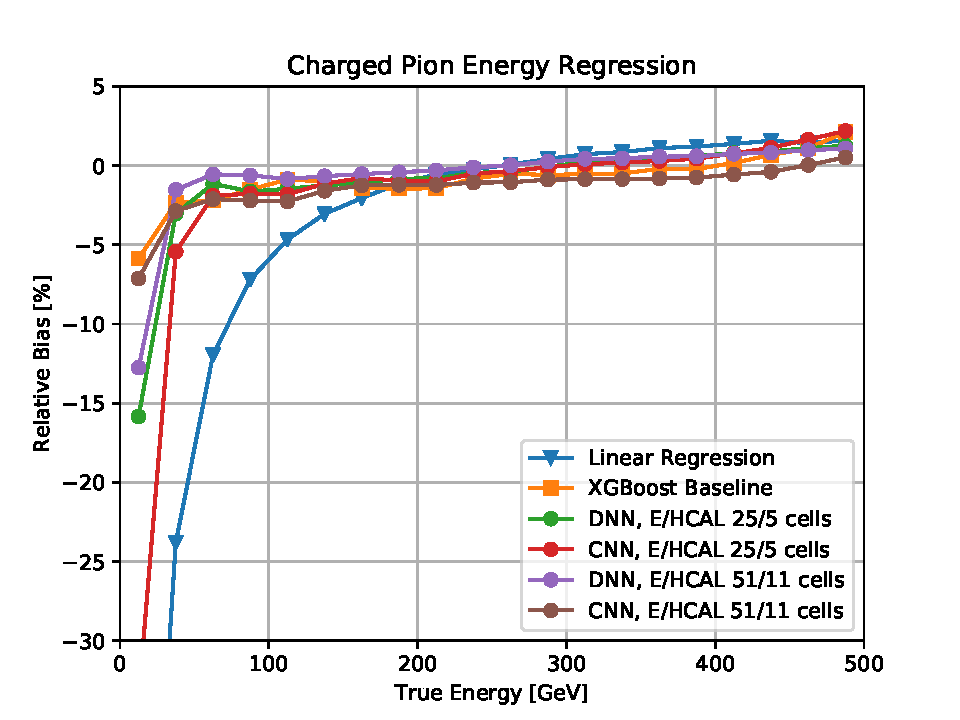
\includegraphics[width=0.38\textwidth]{Images/Calo/bias_vs_E_ChPiFixed_Cut30_nn_numcells.pdf}
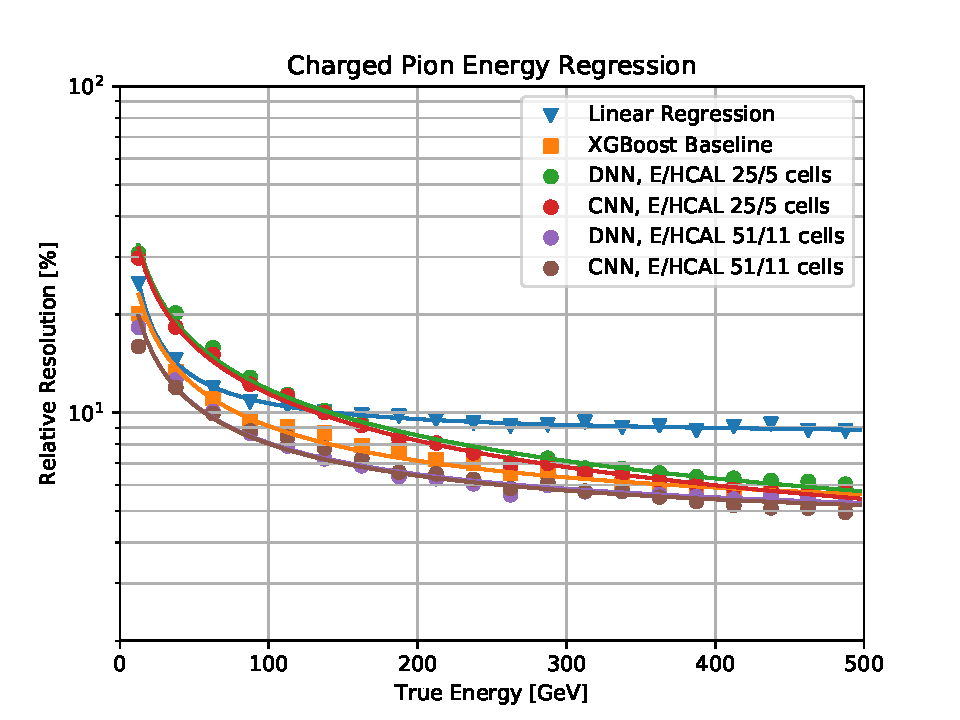
\includegraphics[width=0.38\textwidth]{Images/Calo/res_vs_E_ChPiFixed_Cut30_nn_numcells_fits.pdf}
\caption{Bias (top) and resolution (bottom) as a function of true energy for energy predictions for \chpi, comparing calorimeter window sizes for the CNN and DNN models.
}
\label{fig:reg_nn_numcells_chpi_large_window}
\end{figure}

\subsection*{Skip Connections}

A design choice that improved convergence time, and improved performance for the CNN, is including ``skip connections'' for the total ECAL and HCAL energies in the network.  In addition to the individual cell energy values, the total ECAL and HCAL energy values are given as inputs to both the first dense layer and to the last output layer.  The weights for these energy values are initialized to 1, as linear regression with coefficients near 1 is observed to reasonably reproduce the true energy values.  The impact of adding skip connections on performance using a CNN architecture for a fixed number of 5 training epochs is shown in Figure~\ref{fig:reg_cnn_skip}.

\begin{figure}[htbp]
\centering
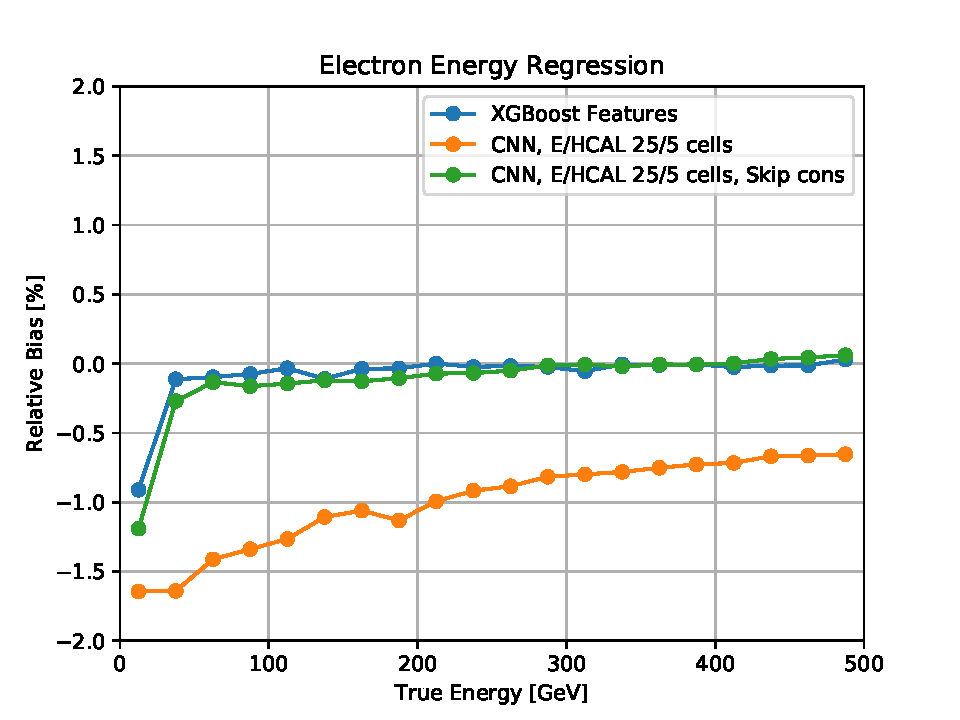
\includegraphics[width=0.38\textwidth]{Images/Calo/bias_vs_E_EleFixed_cnn_skip_zoom.pdf}
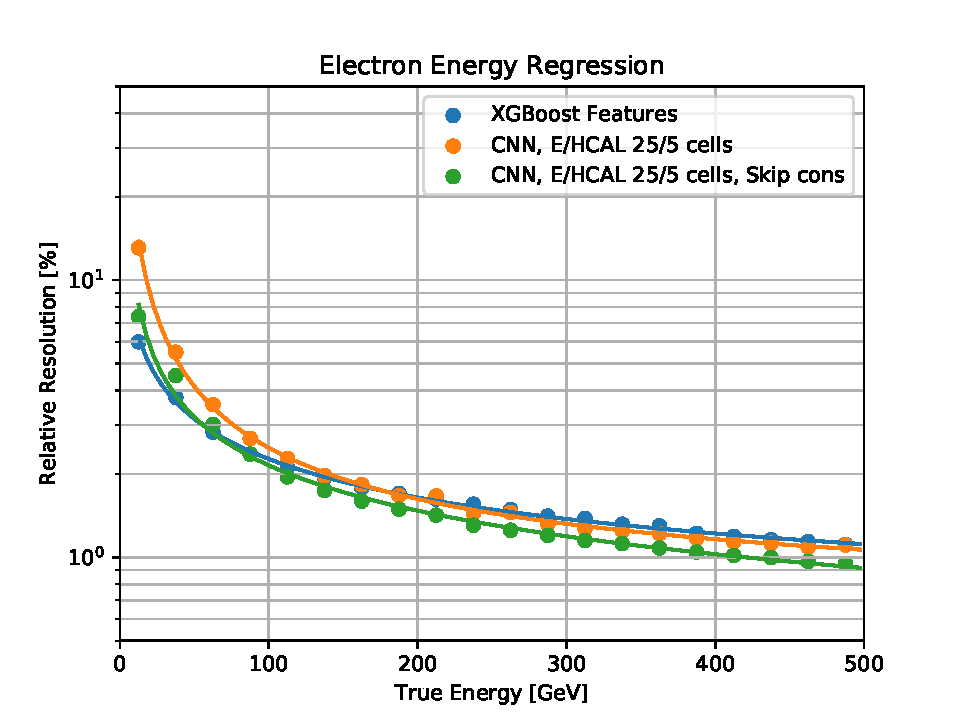
\includegraphics[width=0.38\textwidth]{Images/Calo/res_vs_E_EleFixed_cnn_skip_fits.pdf}
\caption{Bias (top) and resolution (bottom) as a function of true energy for CNN energy predictions for electrons, with or without skip connections in the architecture.
}
\label{fig:reg_cnn_skip}
\end{figure}

\subsection*{Training Using Energy Summed in z}

For regression, we tried using only the energy summed in layers in the $z$ direction, instead of the full array of cell energies, as the mean $z$ coordinate was seen to be the most important additional feature in the XGBoost baseline.  The performance is better than the XGBoost baseline at high energies but worse than using the full cell-level information, as shown in Figure~\ref{fig:reg_dnn_inputs}.

\begin{figure}[htbp]
\centering
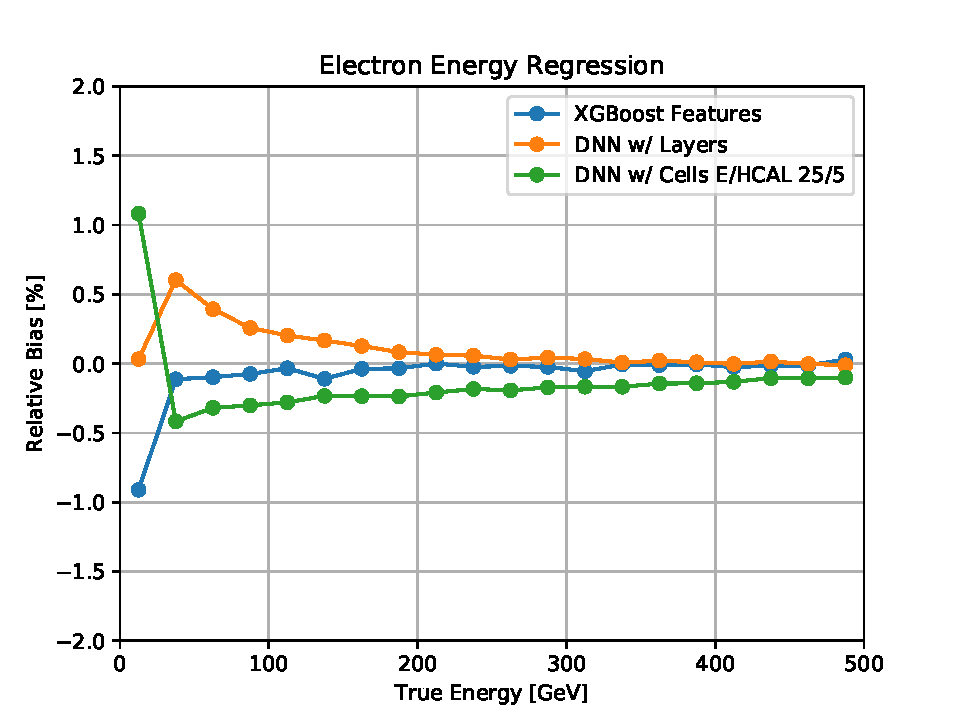
\includegraphics[width=0.38\textwidth]{Images/Calo/bias_vs_E_EleFixed_nn_inputs_zoom.pdf}
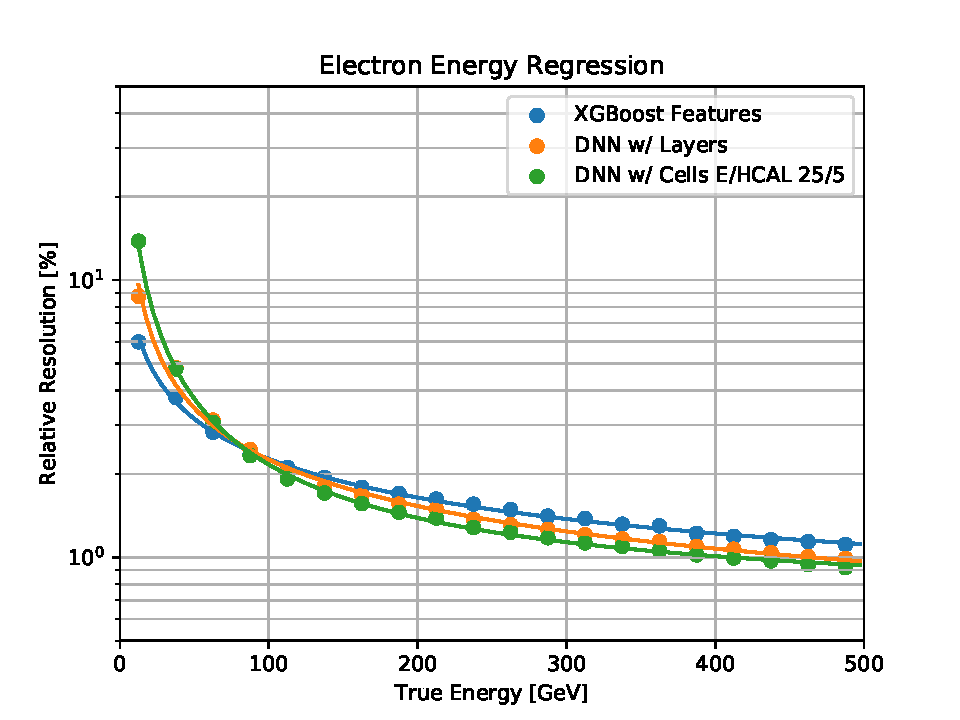
\includegraphics[width=0.38\textwidth]{Images/Calo/res_vs_E_EleFixed_nn_inputs_fits.pdf}
\caption{Bias (top) and resolution (bottom) as a function of true energy for DNN energy predictions for electrons, using as input either the energy summed in layers of $z$, or the full cell information.\label{fig:reg_dnn_inputs}}
\end{figure}

\section{Results}








Updated results for each of the particle types are shown in Figure~\ref{fig:reg_linreg}. Each point in the plot represents the mean bias or resolution within an energy bin. In all the resolution plots shown, the points have been fitted with the expected resolution function of Eq.~\ref{eq:res}, and the fitted function is plotted as a line.

\begin{equation}
\frac{\sigma(\Delta E)}{E_{\text{true}}} = \frac{a}{\sqrt{E_{\text{true}}}} \oplus b \oplus \frac{c}{E_{\text{true}}}
\label{eq:res}
\end{equation}

\begin{figure}[htbp]
\centering
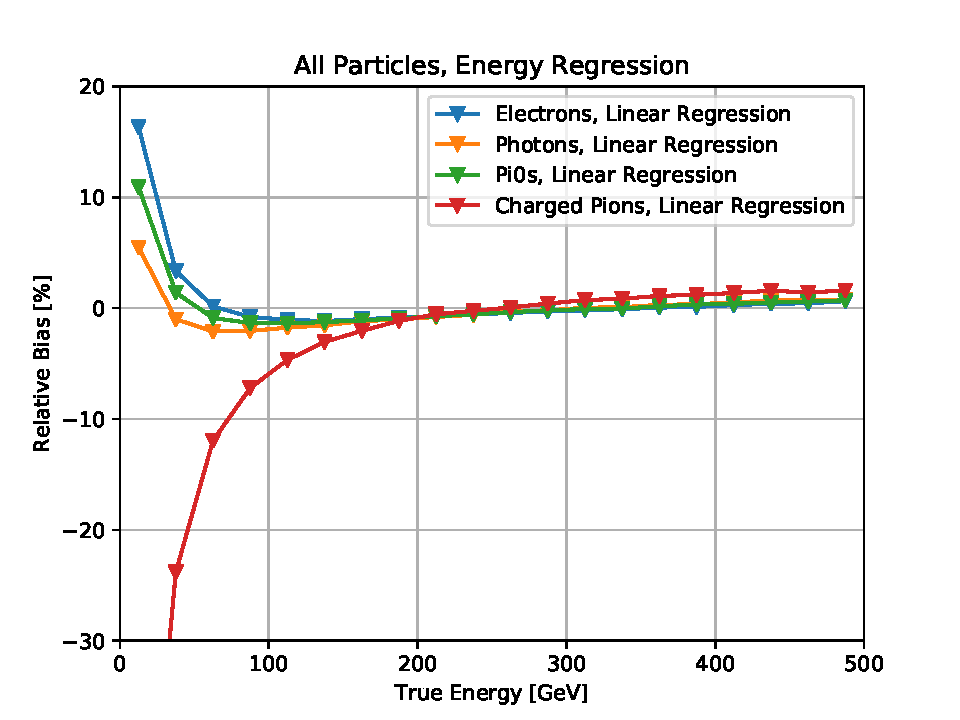
\includegraphics[width=0.38\textwidth]{Images/Calo/bias_vs_E_allparts_linreg.pdf}
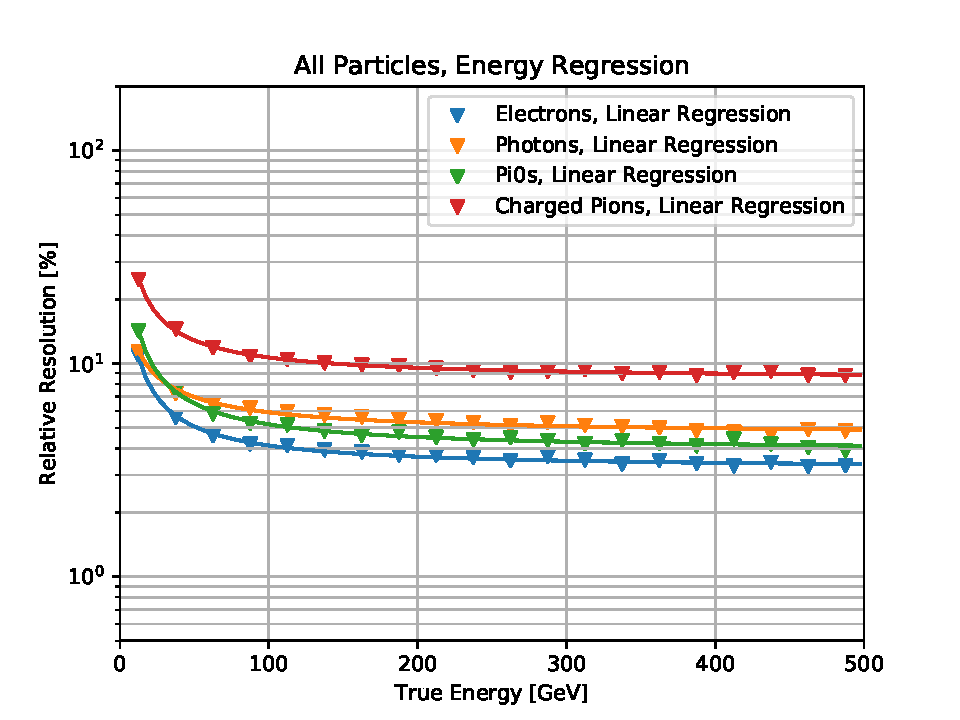
\includegraphics[width=0.38\textwidth]{Images/Calo/res_vs_E_allparts_linreg_fits.pdf}
\caption{Bias (top) and resolution (bottom) as a function of true energy for linear regression predictions of particle energy for the different particle types, trained on fixed-angle samples. \label{fig:reg_linreg}}
\end{figure}






Figure~\ref{fig:reg_dnn_vs_cnn_variable} shows the energy regression performance for each particle type, obtained from the end-to-end reconstruction architectures. In this case, we compare against a linear regression algorithm and a BDT (labelled as "XGBoost") representing the current state-of-the-art, as described in Appendix~\ref{app:regression_baseline}. 

\begin{figure*}[htbp]
\centering
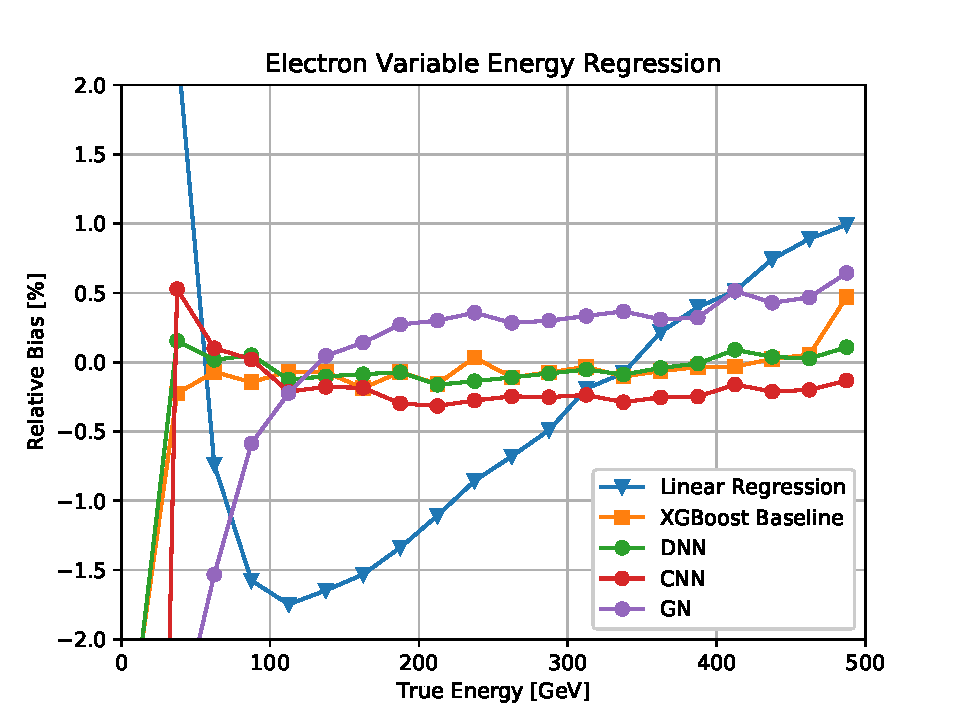
\includegraphics[width=0.38\textwidth]{Images/Calo/bias_vs_E_Ele_variable.pdf}
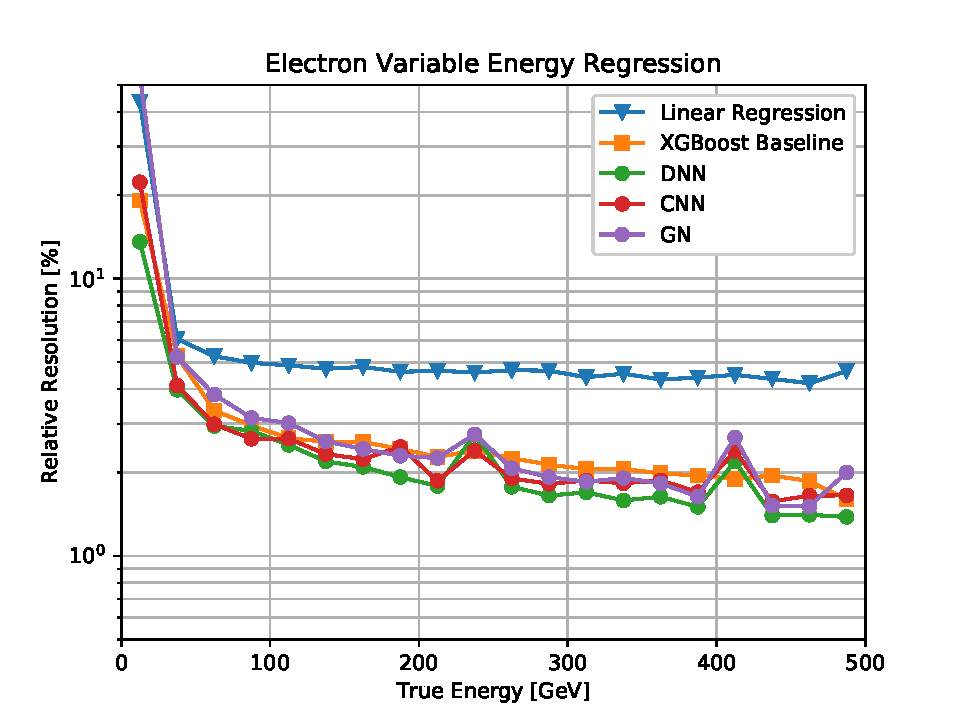
\includegraphics[width=0.38\textwidth]{Images/Calo/res_vs_E_Ele_variable.pdf} \\
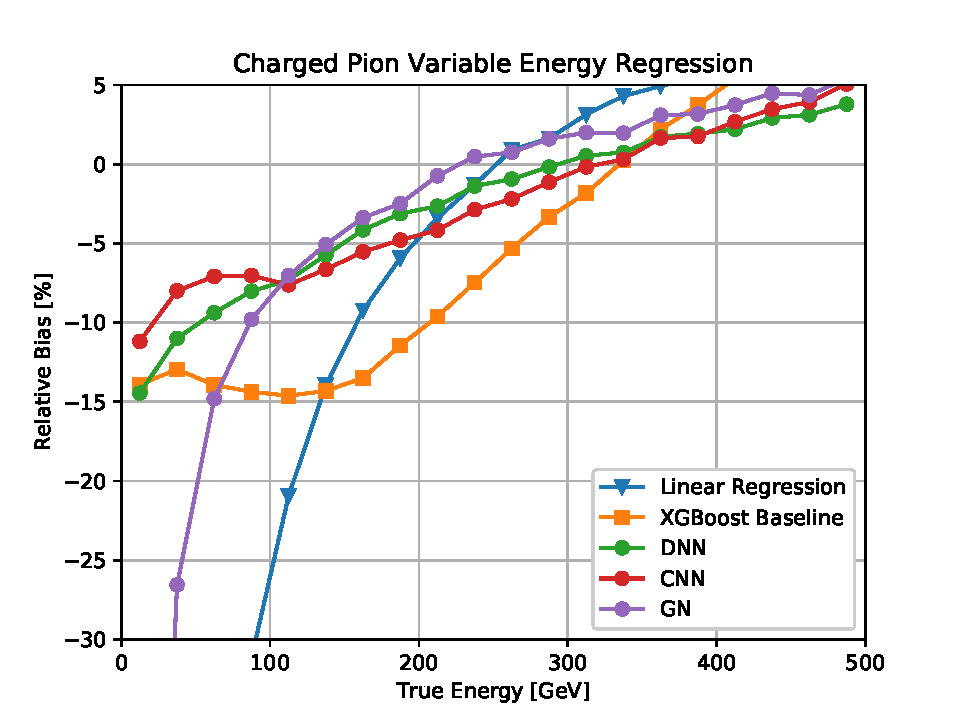
\includegraphics[width=0.38\textwidth]{Images/Calo/bias_vs_E_ChPi_variable.pdf}
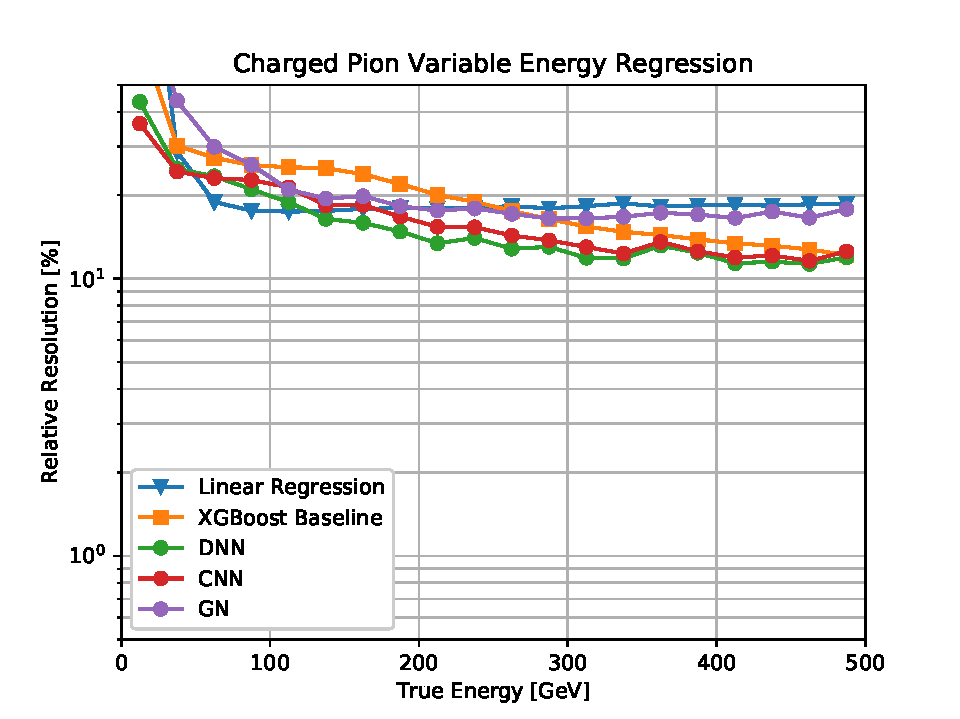
\includegraphics[width=0.38\textwidth]{Images/Calo/res_vs_E_ChPi_variable.pdf} \\
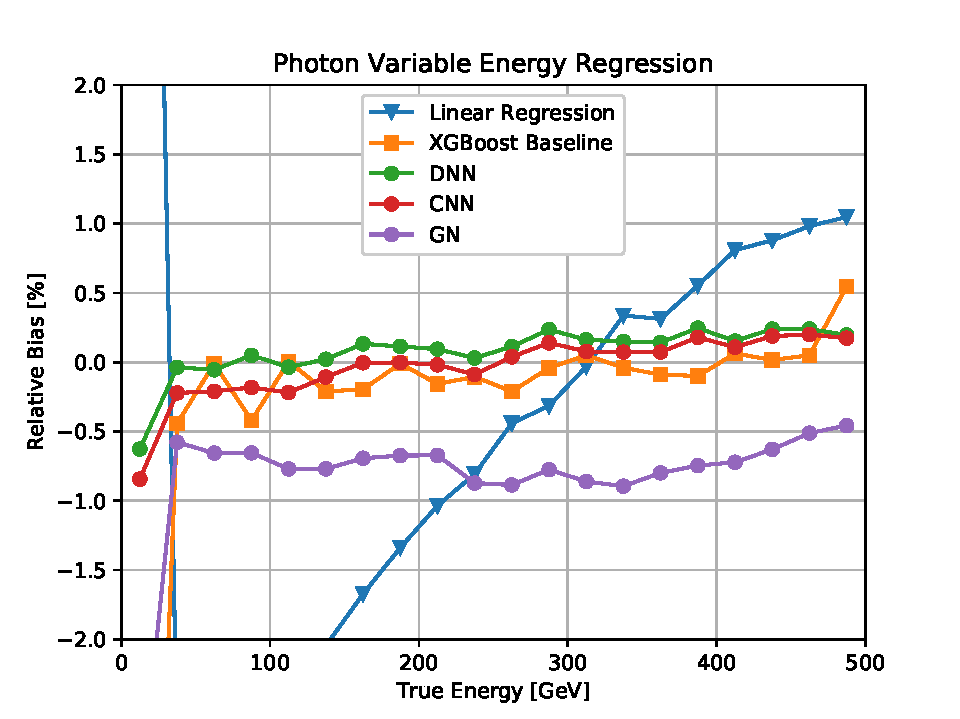
\includegraphics[width=0.38\textwidth]{Images/Calo/bias_vs_E_Gamma_variable.pdf}
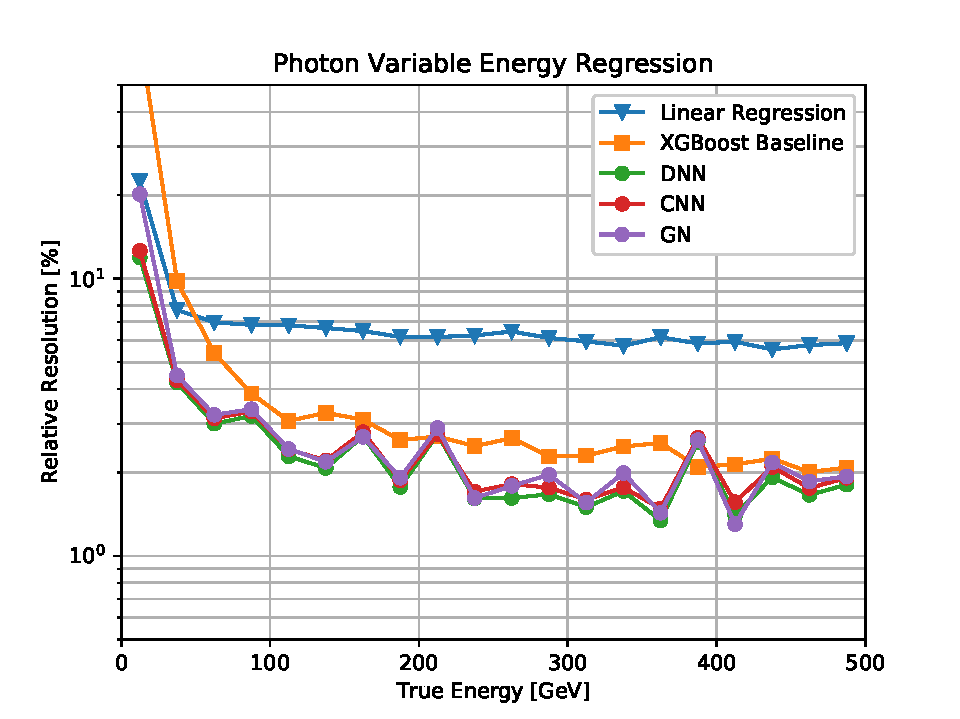
\includegraphics[width=0.38\textwidth]{Images/Calo/res_vs_E_Gamma_variable.pdf}\\
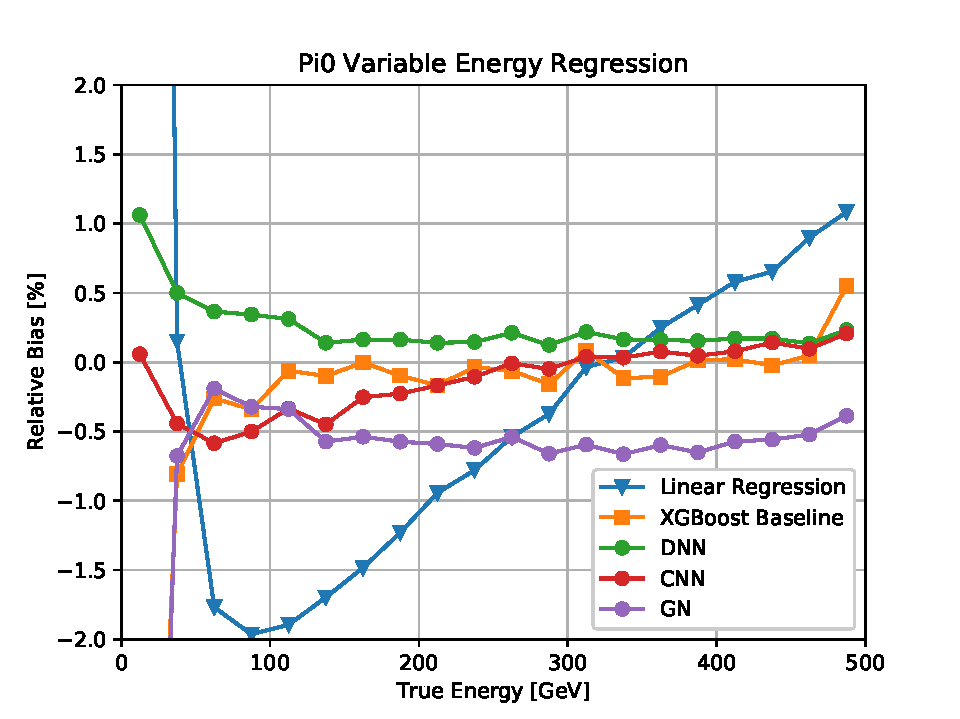
\includegraphics[width=0.38\textwidth]{Images/Calo/bias_vs_E_Pi0_variable.pdf}
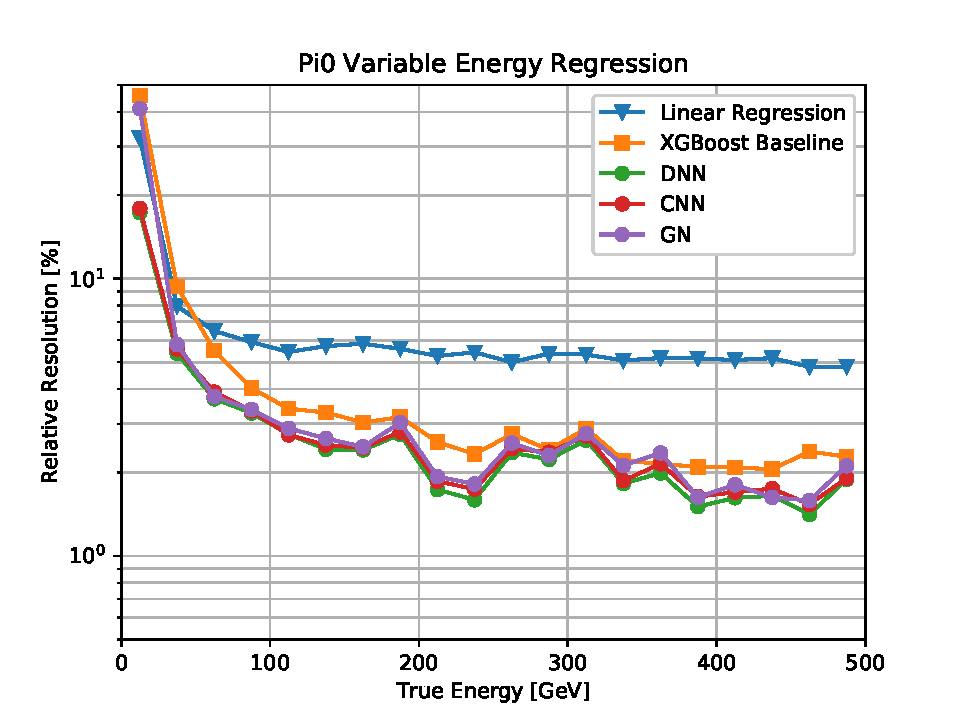
\includegraphics[width=0.38\textwidth]{Images/Calo/res_vs_E_Pi0_variable.pdf}
\caption{Regression bias (left) and resolution (right) as a function
  of true energy for energy predictions on the REC dataset with
  variable-angle incident angle. From top to bottom: electrons,
  charged pions, photons, and neutral
  pions. Algorithms compared are linear regression, XGBoost (BDT), DNN, CNN, and GoogLeNet (GN).\label{fig:reg_dnn_vs_cnn_variable}}
\end{figure*}

Since the energy regression problem is not as complex as the classification problem, the three architectures (DNN, CNN, GN) perform fairly similarly, with the exception of the GN performance on \chpi, which is a bit worse.
%(and possibly slightly over-trained). 
The performance is overall worse for \chpi, both with the networks and with the benchmark baselines (linear regression and XGBoost).

A closer look at the performance boost given by each network can be obtained examining the case of particles entering the calorimeter inner surface at $90^{\mathrm o}$, i.e. with $\eta=0$~\footnote{For these additional fixed-angle regression plots, we did not train GoogLeNet architectures.}. In this case, the problem is more constrained and both the networks and the baseline algorithms are able to perform accurately. The results for fixed angle samples are shown in Appendix~\ref{app:regression_fixed_angle}.

We have also tested the result of training on one class of particle and performing regression on another. These results can be seen in Appendix~\ref{app:xtrain_regression}. In addition, we have looked at the effect on energy regression of increasing the ECAL and HCAL window sizes. This can be seen in Appendix~\ref{app:large_window_regression}.

\subsection*{Cross Training on Different Particle Types}

All the tests so far have assumed that we know exactly what type of particle led to the reconstructed energy deposits.  In a real world situation, the particle identities are not known with complete confidence.  To see how the algorithms above would cope with that situation, we tried training each algorithm on an input sample of electron events, and then we used the trained algorithm to predict the energies for other particle types.

The results are shown in Figure~\ref{fig:reg_nn_cross_gamma} for predicting photon energies and Figure~\ref{fig:reg_nn_cross_pi0} for predicting \pizero\ energies, and are compared to algorithms that are both trained and tested on the same particle type.  In each case, a DNN or CNN trained on electrons is able to achieve the same resolution as a CNN trained on photons or \pizero.  The bias is slightly larger in some cases.

\begin{figure}[hbp]
\centering
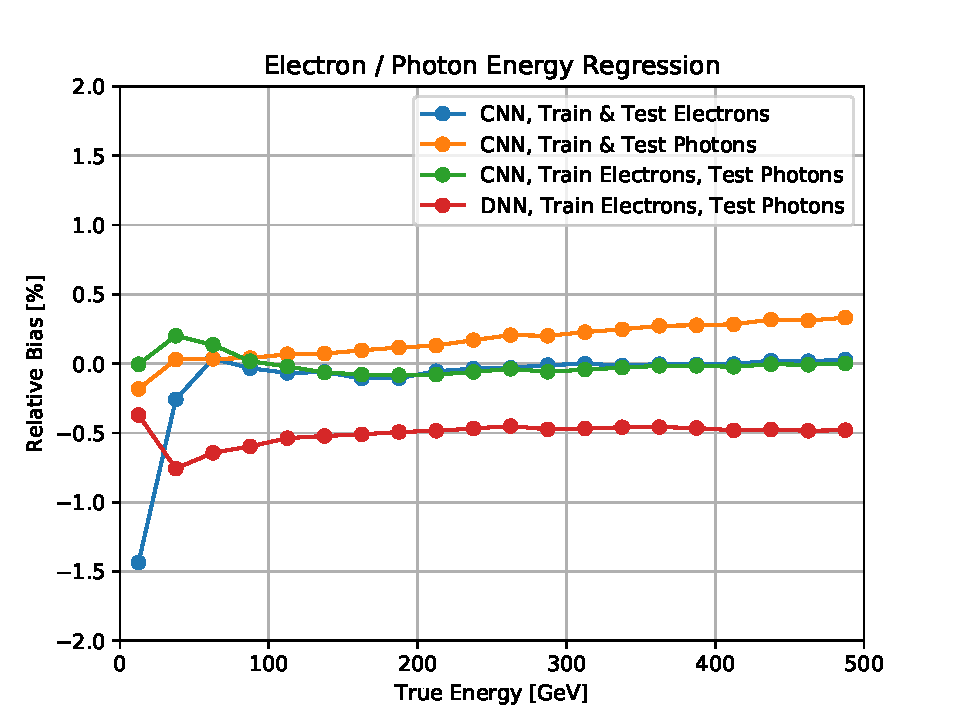
\includegraphics[width=0.38\textwidth]{Images/Calo/bias_vs_E_EleGammaFixed_nn_cross_zoom.pdf}
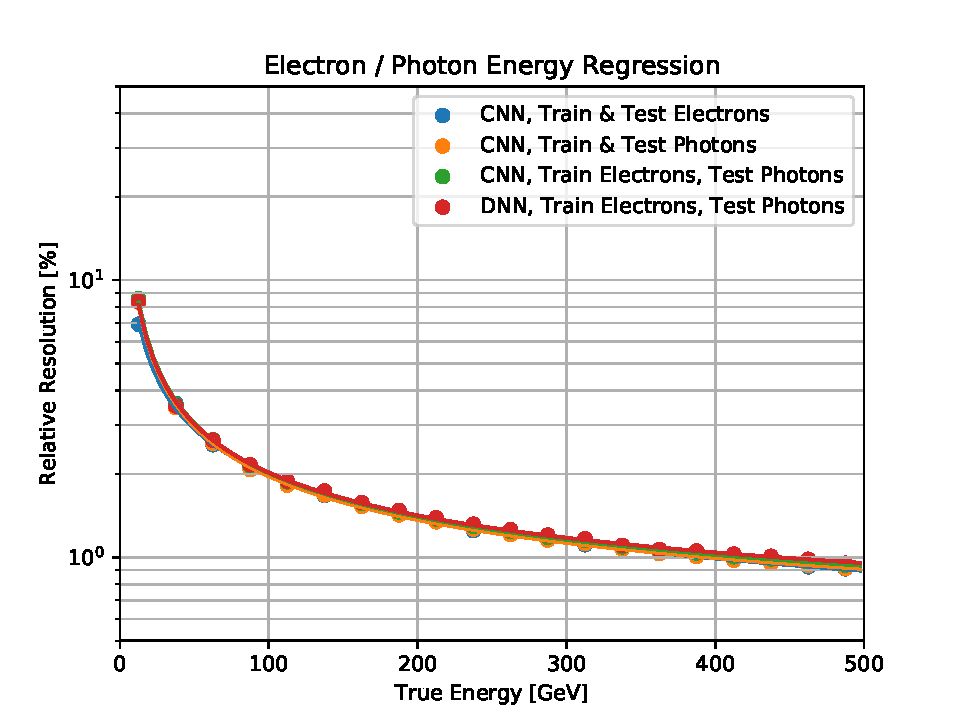
\includegraphics[width=0.38\textwidth]{Images/Calo/res_vs_E_EleGammaFixed_nn_cross_fits.pdf}
\caption{Bias (top) and resolution (bottom) as a function of true energy, for electrons and photons.  The particles used to train and test each algorithm are given in the legend.
}
\label{fig:reg_nn_cross_gamma}
\end{figure}

\begin{figure}[htbp]
\centering
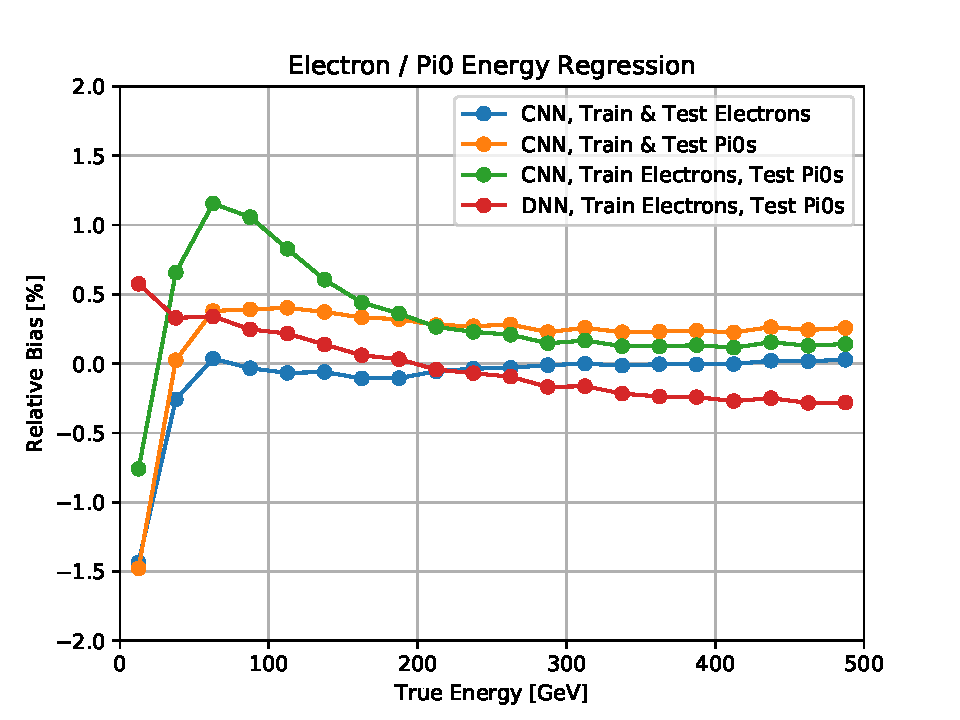
\includegraphics[width=0.38\textwidth]{Images/Calo/bias_vs_E_ElePi0Fixed_nn_cross_zoom.pdf}
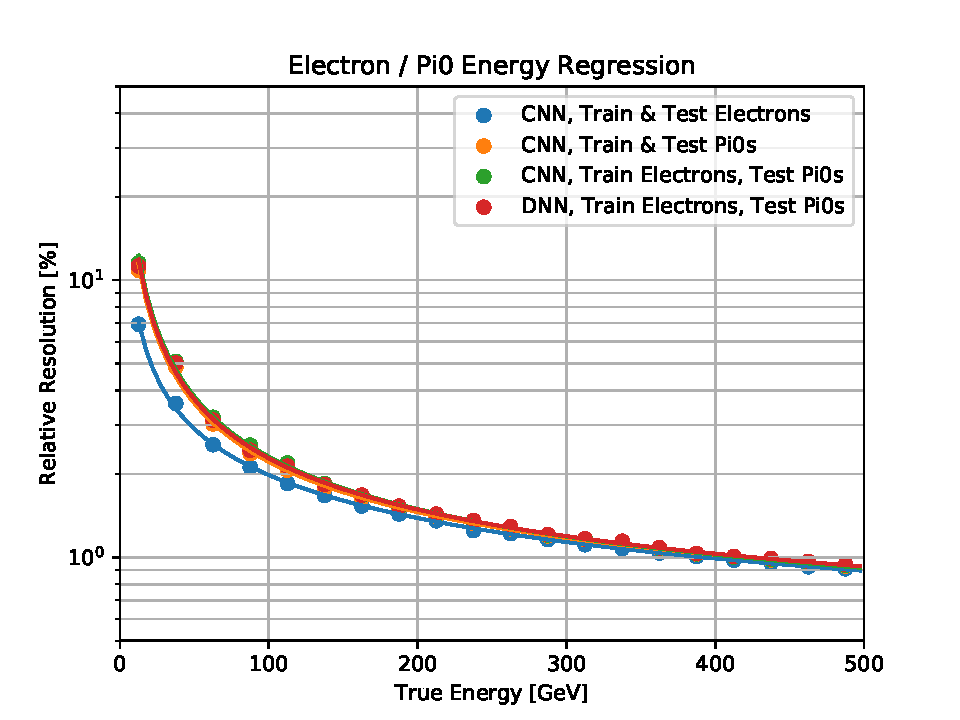
\includegraphics[width=0.38\textwidth]{Images/Calo/res_vs_E_ElePi0Fixed_nn_cross_fits.pdf}
\caption{Bias (top) and resolution (bottom) as a function of true energy, for electrons and \pizero.  The particles used to train and test each algorithm are given in the legend.
}
\label{fig:reg_nn_cross_pi0}
\end{figure}

Models trained on electrons, photons, or \pizero\ were found to not describe \chpi\ well at all.  This is not surprising given that \chpi\ have a hadronic shower, with a large fraction of energy deposited in the HCAL, compared to the other particles depositing almost all of their energy in the ECAL.

We also checked whether the energy regression was different for photons that have converted into an $e^{+}e^{-}$ pair through interaction with the detector material.  These conversion photons comprise about 9\% of the photon sample.  We tried training and/or evaluating regression models separately on converted photons compared to all photons (which are dominated by unconverted).  The results are shown for XGBoost in Figure~\ref{fig:reg_xgb_conv_gamma} and for CNN/DNN models in Figure~\ref{fig:reg_nn_conv_gamma}.  Worse resolution is seen in each case for converted photons below around 100~GeV, which can be attributed to the subsequent electrons forming two showers instead of one in the calorimeter.  With XGBoost, the resolution remains the same for converted photons when training on the full sample, while for CNN or DNN, the resolution is worse below around 100~GeV.  The bias is also worse for converted photons at lower energy when training on all photons.

\begin{figure}[htbp]
\centering
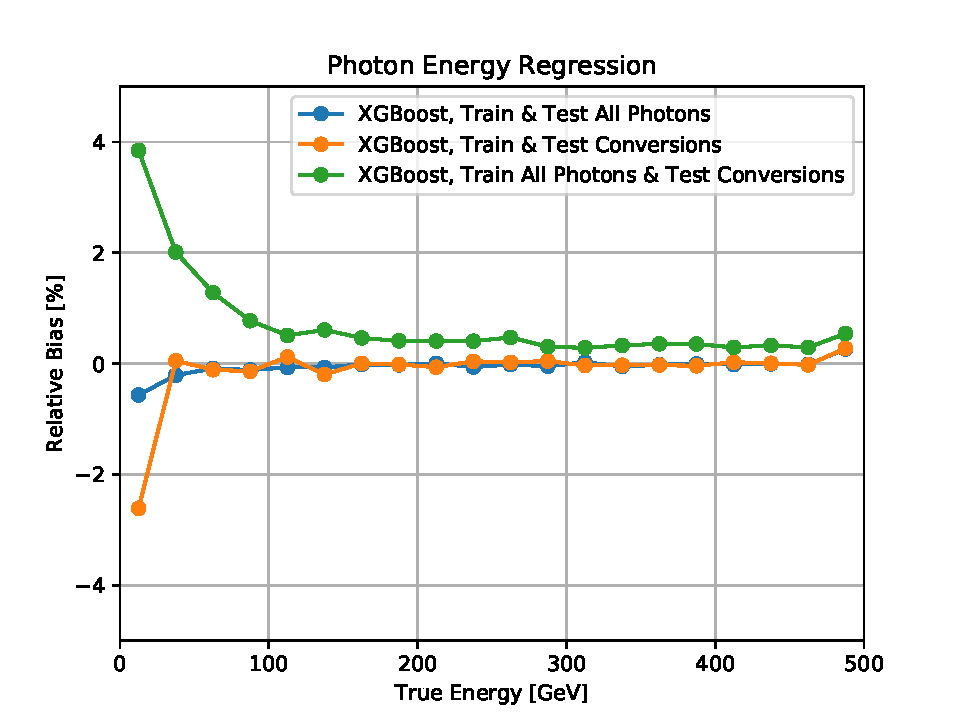
\includegraphics[width=0.38\textwidth]{Images/Calo/bias_vs_E_GammaFixed_xgb_convs.pdf}
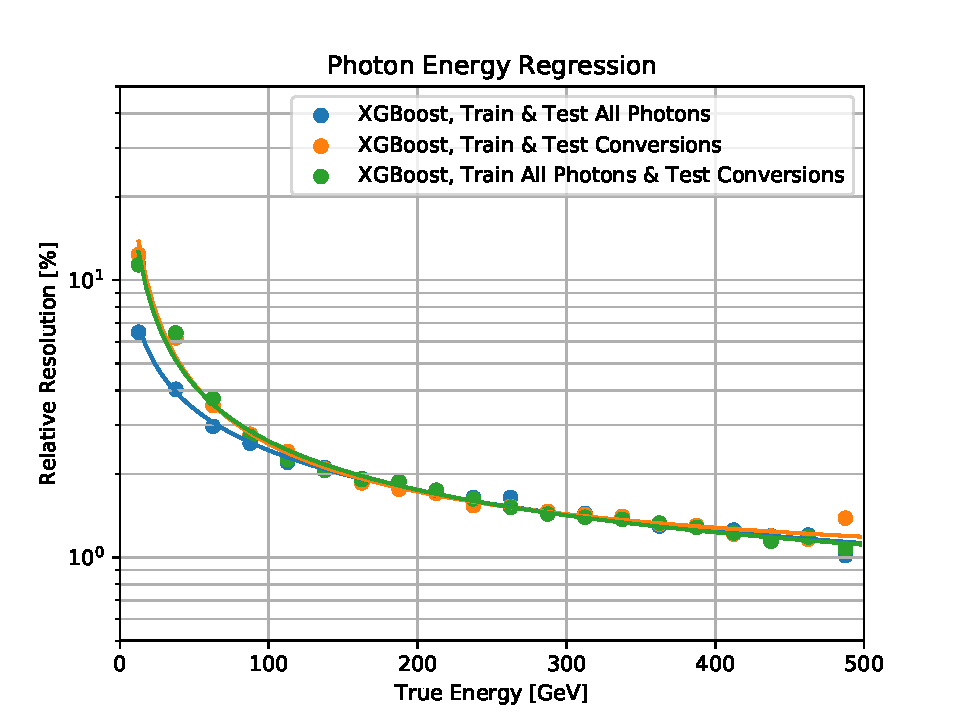
\includegraphics[width=0.38\textwidth]{Images/Calo/res_vs_E_GammaFixed_xgb_convs_fits.pdf}
\caption{Bias (top) and resolution (bottom) as a function of true energy, for photons using XGBoost regression.  We look at the photon sample when split up by conversions.
}
\label{fig:reg_xgb_conv_gamma}
\end{figure}

\begin{figure}[htbp]
\centering
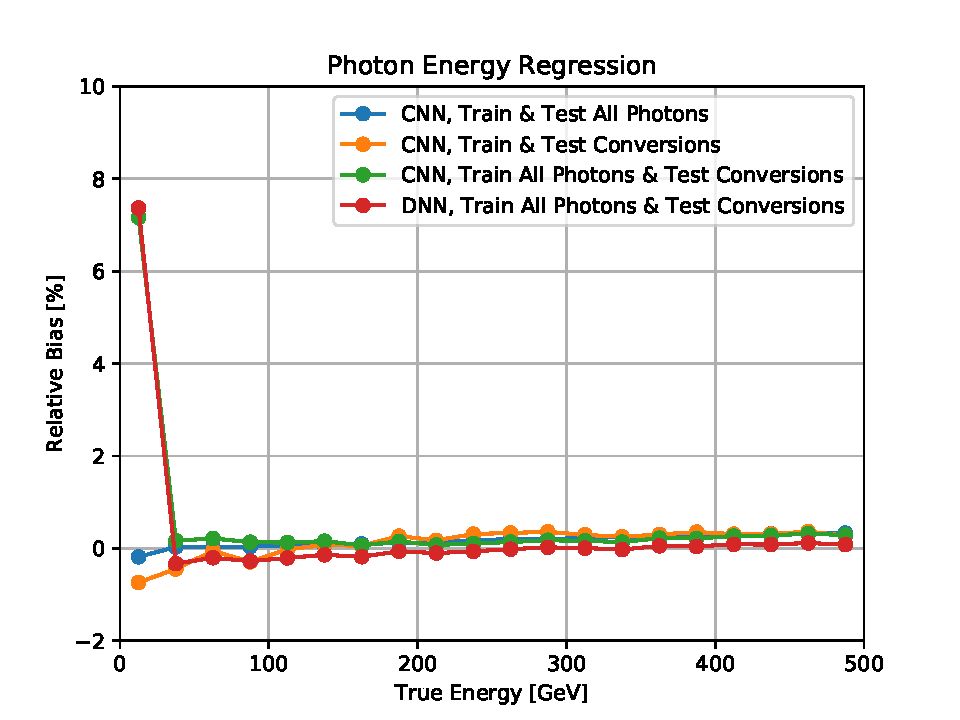
\includegraphics[width=0.38\textwidth]{Images/Calo/bias_vs_E_GammaFixed_nn_convs.pdf}
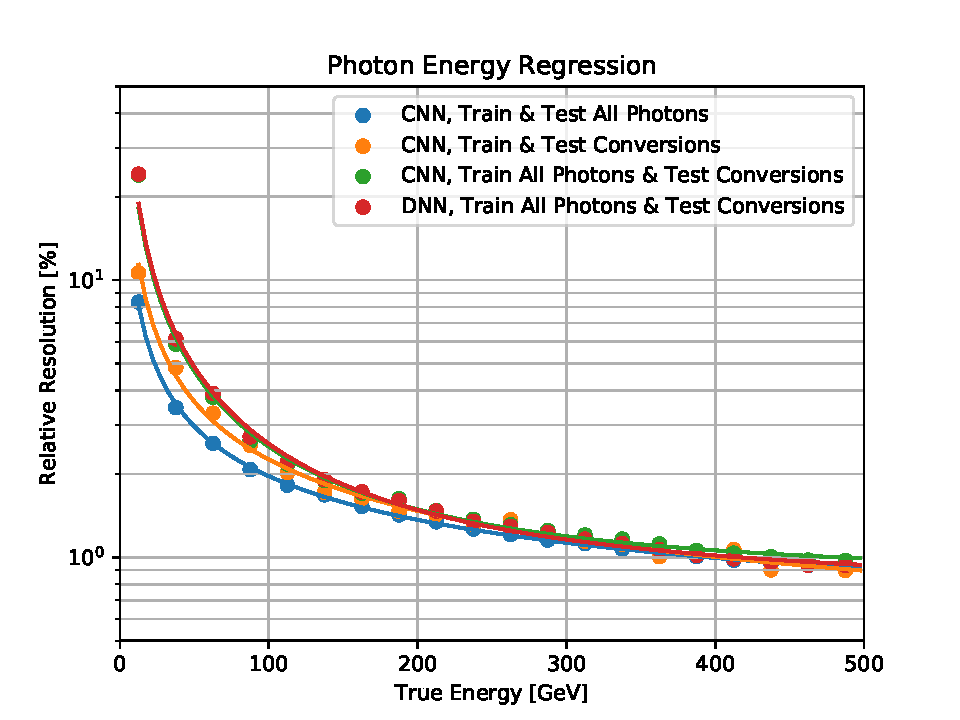
\includegraphics[width=0.38\textwidth]{Images/Calo/res_vs_E_GammaFixed_nn_convs_fits.pdf}
\caption{Bias (top) and resolution (bottom) as a function of true energy, for photons using CNN or DNN regression.  We look at the photon sample when split up by conversions.
}
\label{fig:reg_nn_conv_gamma}
\end{figure}